%!TEX TS-program = xelatex

% Шаблон документа LaTeX создан в 2018 году
% Алексеем Подчезерцевым
% В качестве исходных использованы шаблоны
% 	Данилом Фёдоровых (danil@fedorovykh.ru) 
%		https://www.writelatex.com/coursera/latex/5.2.2
%	LaTeX-шаблон для русской кандидатской диссертации и её автореферата.
%		https://github.com/AndreyAkinshin/Russian-Phd-LaTeX-Dissertation-Template

\documentclass[a4paper,14pt]{article}


%%% Работа с русским языком
\usepackage[english,russian]{babel}   %% загружает пакет многоязыковой вёрстки
\usepackage{fontspec}      %% подготавливает загрузку шрифтов Open Type, True Type и др.
\defaultfontfeatures{Ligatures={TeX},Renderer=Basic}  %% свойства шрифтов по умолчанию
\setmainfont[Ligatures={TeX,Historic}]{Times New Roman} %% задаёт основной шрифт документа
\setsansfont{Comic Sans MS}                    %% задаёт шрифт без засечек
\setmonofont{Courier New}
\usepackage{indentfirst}
\frenchspacing

\renewcommand{\epsilon}{\ensuremath{\varepsilon}}
\renewcommand{\phi}{\ensuremath{\varphi}}
\renewcommand{\kappa}{\ensuremath{\varkappa}}
\renewcommand{\le}{\ensuremath{\leqslant}}
\renewcommand{\leq}{\ensuremath{\leqslant}}
\renewcommand{\ge}{\ensuremath{\geqslant}}
\renewcommand{\geq}{\ensuremath{\geqslant}}
\renewcommand{\emptyset}{\varnothing}

%%% Дополнительная работа с математикой
\usepackage{amsmath,amsfonts,amssymb,amsthm,mathtools} % AMS
\usepackage{icomma} % "Умная" запятая: $0,2$ --- число, $0, 2$ --- перечисление

%% Номера формул
%\mathtoolsset{showonlyrefs=true} % Показывать номера только у тех формул, на которые есть \eqref{} в тексте.
%\usepackage{leqno} % Нумерация формул слева	

%% Перенос знаков в формулах (по Львовскому)
\newcommand*{\hm}[1]{#1\nobreak\discretionary{}
	{\hbox{$\mathsurround=0pt #1$}}{}}

%%% Работа с картинками
\usepackage{graphicx}  % Для вставки рисунков
\graphicspath{{images/}}  % папки с картинками
\setlength\fboxsep{3pt} % Отступ рамки \fbox{} от рисунка
\setlength\fboxrule{1pt} % Толщина линий рамки \fbox{}
\usepackage{wrapfig} % Обтекание рисунков текстом

%%% Работа с таблицами
\usepackage{array,tabularx,tabulary,booktabs} % Дополнительная работа с таблицами
\usepackage{longtable}  % Длинные таблицы
\usepackage{multirow} % Слияние строк в таблице
\usepackage{float}% http://ctan.org/pkg/float

%%% Программирование
\usepackage{etoolbox} % логические операторы


%%% Страница
\usepackage{extsizes} % Возможность сделать 14-й шрифт
\usepackage{geometry} % Простой способ задавать поля
\geometry{top=20mm}
\geometry{bottom=20mm}
\geometry{left=20mm}
\geometry{right=10mm}
%
%\usepackage{fancyhdr} % Колонтитулы
% 	\pagestyle{fancy}
%\renewcommand{\headrulewidth}{0pt}  % Толщина линейки, отчеркивающей верхний колонтитул
% 	\lfoot{Нижний левый}
% 	\rfoot{Нижний правый}
% 	\rhead{Верхний правый}
% 	\chead{Верхний в центре}
% 	\lhead{Верхний левый}
%	\cfoot{Нижний в центре} % По умолчанию здесь номер страницы

\usepackage{setspace} % Интерлиньяж
\onehalfspacing % Интерлиньяж 1.5
%\doublespacing % Интерлиньяж 2
%\singlespacing % Интерлиньяж 1

\usepackage{lastpage} % Узнать, сколько всего страниц в документе.

\usepackage{soul} % Модификаторы начертания

\usepackage{hyperref}
\usepackage[usenames,dvipsnames,svgnames,table,rgb]{xcolor}
\hypersetup{				% Гиперссылки
	unicode=true,           % русские буквы в раздела PDF
	pdftitle={Заголовок},   % Заголовок
	pdfauthor={Автор},      % Автор
	pdfsubject={Тема},      % Тема
	pdfcreator={Создатель}, % Создатель
	pdfproducer={Производитель}, % Производитель
	pdfkeywords={keyword1} {key2} {key3}, % Ключевые слова
	colorlinks=true,       	% false: ссылки в рамках; true: цветные ссылки
	linkcolor=black,          % внутренние ссылки
	citecolor=black,        % на библиографию
	filecolor=magenta,      % на файлы
	urlcolor=black           % на URL
}
\makeatletter 
\def\@biblabel#1{#1. } 
\makeatother
\usepackage{cite} % Работа с библиографией
%\usepackage[superscript]{cite} % Ссылки в верхних индексах
%\usepackage[nocompress]{cite} % 
\usepackage{csquotes} % Еще инструменты для ссылок

\usepackage{multicol} % Несколько колонок

\usepackage{tikz} % Работа с графикой
\usepackage{pgfplots}
\usepackage{pgfplotstable}

% ГОСТ заголовки
\usepackage[font=small]{caption}
%\captionsetup[table]{justification=centering, labelsep = newline} % Таблицы по правобу краю
%\captionsetup[figure]{justification=centering} % Картинки по центру


\newcommand{\tablecaption}[1]{\addtocounter{table}{1}\small \begin{flushright}\tablename \ \thetable\end{flushright}%	
\begin{center}#1\end{center}}

\newcommand{\imref}[1]{рис.~\ref{#1}}

\usepackage{multirow}
\usepackage{spreadtab}
\newcolumntype{K}[1]{@{}>{\centering\arraybackslash}p{#1cm}@{}}


\usepackage{xparse}
\usepackage{fancyvrb}

\RecustomVerbatimCommand{\VerbatimInput}{VerbatimInput}
{
	fontsize=\footnotesize    
}

\usepackage{tocloft}
\renewcommand{\cftsecleader}{\cftdotfill{\cftdotsep}}
\begin{document} % конец преамбулы, начало документа
	\begin{titlepage}
	\begin{center}
 		ФЕДЕРАЛЬНОЕ  ГОСУДАРСТВЕННОЕ АВТОНОМНОЕ \\
		ОБРАЗОВАТЕЛЬНОЕ УЧРЕЖДЕНИЕ ВЫСШЕГО ОБРАЗОВАНИЯ\\
		«НАЦИОНАЛЬНЫЙ ИССЛЕДОВАТЕЛЬСКИЙ УНИВЕРСИТЕТ\\
		«ВЫСШАЯ ШКОЛА ЭКОНОМИКИ»
	\end{center}
	
	\begin{center}
		\textbf{Московский институт электроники и математики}
		
		\textbf{им. А.Н.Тихонова НИУ ВШЭ}
		
		\vspace{2ex}
		
		\textbf{Департамент компьютерной инженерии}
	\end{center}
	\vspace{1ex}	
	
	\begin{center}
	\textbf{ОТЧЕТ\\
		ПО ЛАБОРАТОРНОЙ РАБОТЕ №6
	}
	\end{center}	
	\vspace{2ex}
	\begin{center}
		по дисциплине «Проектирование систем на кристалле»
	\end{center}	

	\vspace{2ex}

	\begin{flushright}
		\textbf{Выполнили:}
		
		\vspace{2ex}
		
		Студенты группы БИВ174
		
		Бригада №5
		
		\vspace{2ex}
		
		Подчезерцев Алексей Евгеньевич
		
		Солодянкин Андрей Александрович
		\vspace{2ex}
		
	\end{flushright}

	\vfill
	\begin{center}
		Москва \the\year \, г.
	\end{center}
	
\end{titlepage}
\addtocounter{page}{1}
	\tableofcontents
	\pagebreak
	\section{Задание}
	
	\begin{enumerate}
		\item Сравните временную диаграмму симуляционной модели с диаграммой сигналов из документации на микросхему.
		\item \begin{itemize}
			\item Используя шаги, описанные в Разделе 9.2.5, запустите симуляцию примера 01\_badstyle. Не закрывайте окно симулятора;
			\item Откройте документацию на АЦП ADC081S021 и сравните временную диаграмму в окне симулятора с временной диаграммой из документации;
			\item В среде Quartus Prime откройте пункт меню Tools -> Netlist Viewers -> RTL Viewer;
			\item Найдите экземпляр модуля делителя частоты и сравните его с представленным на Рисунке 9.18;
			\item В среде Quartus Prime откройте пункт меню Tools -> Netlist Viewers -> State Machine	Viewer. Этот же результат можно получить двойным щелчком мыши на желтом прямоугольнике конечного автомата внутри окна RТL Viewer;
			\item Сравните диаграмму конечного автомата с вариантом, разработанным на этапе	проектирования (Рисунок 9.15, Рисунок 9.17);
			\item Откройте файл 01\_badstyle/pmod\_als.v в текстовом редакторе;
			\item Сравните этот код с блок-схемами конечных автоматов (Рисунок 9.1, Рисунок 9.2).
		\end{itemize}
	\end{enumerate}
	
	\section{Дополнительные задания}
	
	\subsection{Задание 1}
	
	Сравните временную диаграмму симуляционной модели с	диаграммой сигналов из документации на микросхему. 		
	
	На рис. \ref{fig:9.7} приведена временная диаграмма из документации к микросхеме ADC081S021, на рис. \ref{fig:9.11} диаграмма симуляционной модели микросхемы.
	
	\begin{figure}[H]
		\centering
		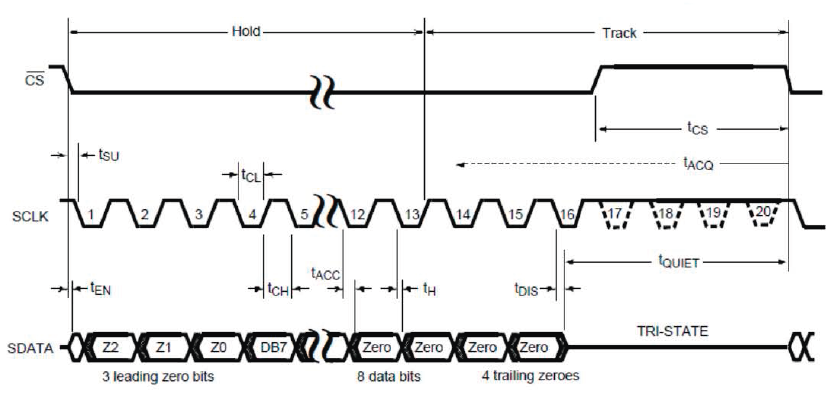
\includegraphics[width=0.9\linewidth]{images/9_7}
		\caption{ADC081S021 Временная диаграмма обмена данными из документации}
		\label{fig:9.7}
	\end{figure}
	
	
	\begin{figure}[H]
		\centering
		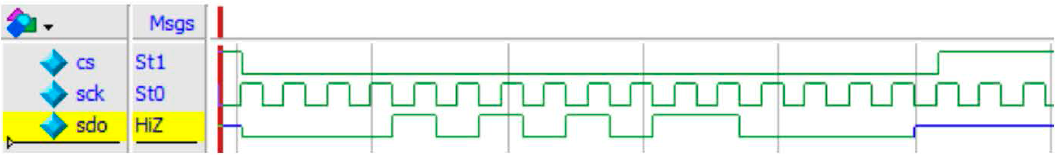
\includegraphics[width=0.9\linewidth]{images/9_11}
		\caption{Временная диаграмма симуляционной модели микросхемы ADC081S021}
		\label{fig:9.11}
	\end{figure}

	На обеих временных диаграммах изображены 3 временные характеристики: $cs$ - chip select, сигнал выбора микросхемы, $sclk(sck)$ - тактовый импульс, $sdata(sdo)$ - slave data out, данные, получаемые из микросхемы.
	
	$sclk(sck)$ мало чем может отличаться, т.к. это тактовый импульс.
	
	$cs$ на обоих графиках установлен в значение логического нуля на протяжении 16 импульсов.
	
	$sdata(sdo)$ на обоих графиках меняет свое состояние по заднему фронту тактового импульса. При этом после первых трех тактовых импульсов наблюдаются нулевые биты, далее идут 8 информационных битов, далее идут 4 нулевых бита и после 16 тактового импульса сигнал принимает высокоимпедансное состояние.
	
	Разница в графиках только в длительности фронтов.	
	
	\subsection{Задание 2}

	После запуска симуляции в modelSim была получена диаграмма, представленная на рис. \ref{fig:z15msimwvf}.
	
	\begin{figure}[H]
		\centering
		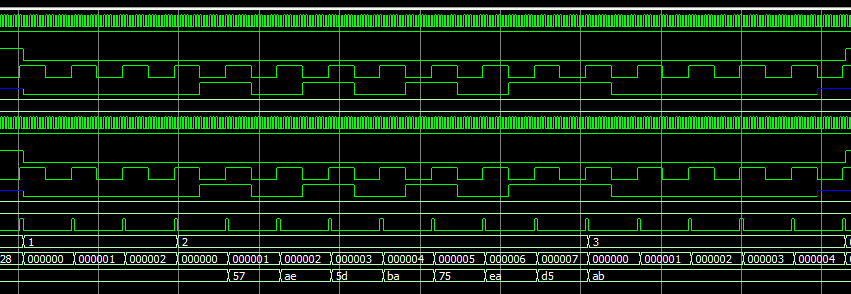
\includegraphics[width=0.9\linewidth]{images/z1_5_msim_wvf}
		\caption{Временная диаграмма для 01\_badstyle}
		\label{fig:z15msimwvf}
	\end{figure}

	При сравнении диаграмм (рис. \ref{fig:9.7} и рис. \ref{fig:z15msimwvf}) видно, что микросхема ADC081S021 реализована верно. Их сравнение аналогично сравнению в задании 1.
	
	На рис. \ref{fig:z15rtl} RTL представление менеджера сессий для 01\_badstyle.
	
	\begin{figure}[H]
		\centering
		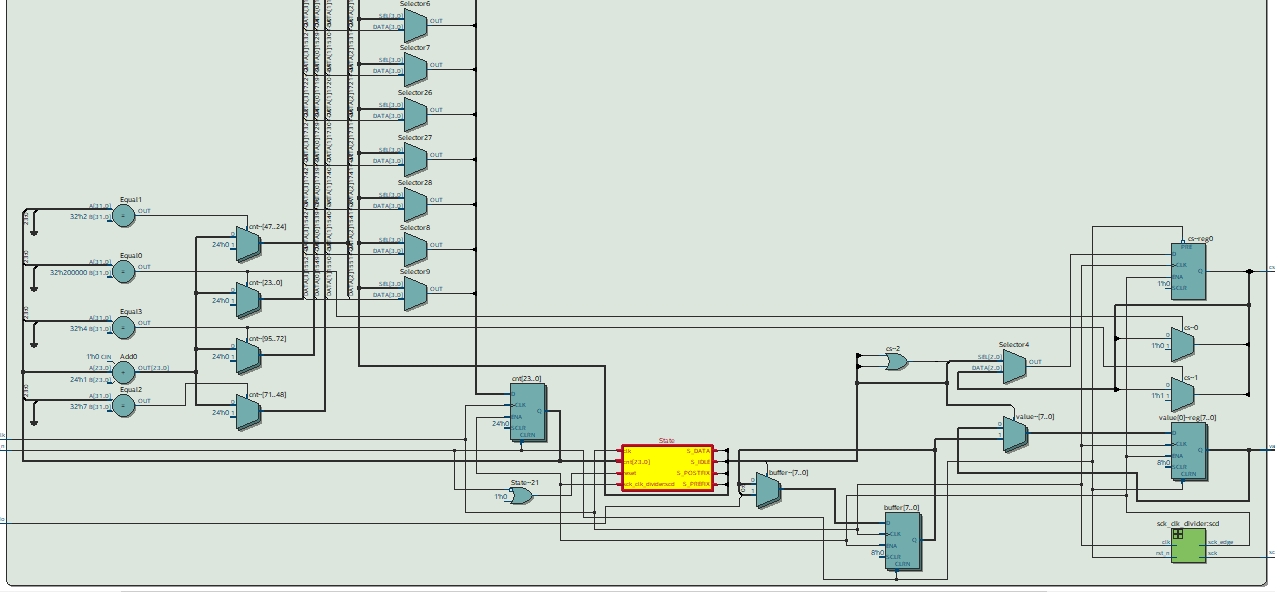
\includegraphics[width=0.9\linewidth]{images/z1_5_rtl}
		\caption{RTL представление менеджера сессий для 01\_badstyle}
		\label{fig:z15rtl}
	\end{figure}

	На рис. \ref{fig:z15rtlclkdivider} RTL представление делителя частоты для 01\_badstyle.
	
	\begin{figure}[H]
		\centering
		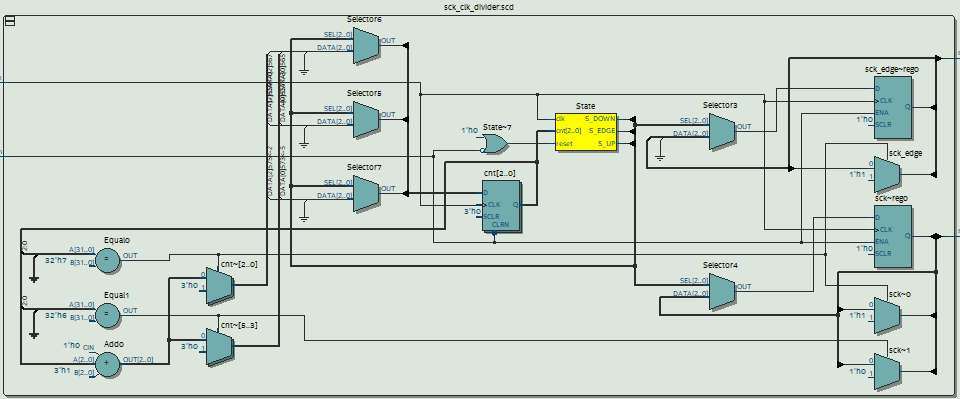
\includegraphics[width=0.9\linewidth]{images/z1_5_rtl_clk_divider}
		\caption{RTL представление делителя частоты для 01\_badstyle}
		\label{fig:z15rtlclkdivider}
	\end{figure}

	На рис. \ref{fig:z15auto} диаграмма состояний менеджера сессий для 01\_badstyle.
	
	\begin{figure}[H]
		\centering
		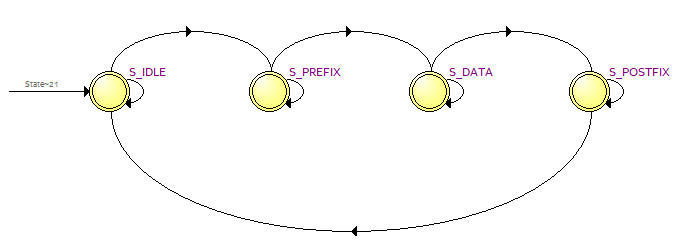
\includegraphics[width=0.6\linewidth]{images/z1_5_auto}
		\caption{Диаграмма состояний менеджера сессий для 01\_badstyle}
		\label{fig:z15auto}
	\end{figure}
	
	На рис. \ref{fig:z15autoclkdivider} диаграмма состояний делителя частоты для 01\_badstyle.
	
	\begin{figure}[H]
		\centering
		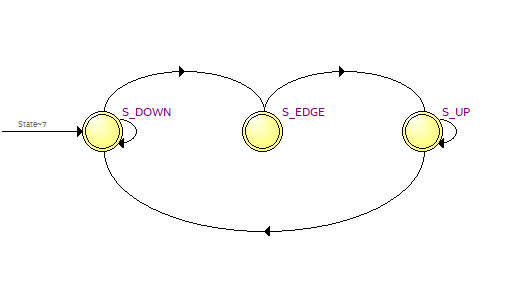
\includegraphics[width=0.6\linewidth]{images/z1_5_auto_clk_divider}
		\caption{Диаграмма состояний делителя частоты для 01\_badstyle}
		\label{fig:z15autoclkdivider}
	\end{figure}

	Все диаграммы совпадают с диаграммами представленными в методичке.
	
	Данный кусок кода описывает схему переходов для менеджера сессий.
	
	{\small \VerbatimInput{verilog/z1_5_men_sess.v}}

	Данный кусок кода описывает схему переходов для делителя частоты.
	
	{\small \VerbatimInput{verilog/z1_5_clk_divider.v}}
	\section{Задания для самостоятельной работы}

	\subsection{Задание 1}

	\section{Контрольные вопросы}
	
	\begin{enumerate}
		
		\item   
	\end{enumerate}
	
	\section{Выводы по работе}
	
	В ходе работы получен опыт проектирования схем в программе Quartus с помощью языка Verilog.
	Полученное устройство было протестировано с помощью бенчтестов в программе Quartus Simulation Waveform editor.
	В процессе работы были смоделированы конечные автоматы Мура и Мили.
	%В процессе работы были смоделированы различные шифраторы и дешифраторы, протестированы способы оптимизации схемы, а так же рассчитаны временные параметры схемы с различными способами оптимизации.
	В процессе был получен опыт работы с платой DE10-Lite, на которой проверялась работоспособность полученного устройства.
	
	\newpage 
	\renewcommand{\refname}{{\normalsize Список использованных источников}} 
	\centering 
	\begin{thebibliography}{9} 
		\addcontentsline{toc}{section}{\refname} 
		\bibitem{Verilog} Thomas D., Moorby P. The Verilog Hardware Description Language. – Springer Science \& Business Media, 2008.
		\bibitem{citekey} Khor W. Y. et al. Evaluation of FPGA Based QSPI Flash Access Using Partial Reconfiguration //2019 7th International Conference on Smart Computing \& Communications (ICSCC). – IEEE, 2019. – С. 1-5
	\end{thebibliography}
	
\end{document} % конец документа
